Computational complexity for estimating I-prior models (and in fact, for GPR in general) is dominated by the inversion (by way of eigendecomposition in our case) of the $n \times n$ matrix $\bSigma_\theta = \psi\bH_\eta^2 + \psi^{-1}\bI_n$, which scales as $O(n^3)$ in time.
%Inversion by way of the eigendecomposition of $\bH_\eta$ is $O(n^3)$.
For the direct optimisation method, this matrix inversion is called when computing the log-likelihood, and thus must be computed at each Newton step.
For the EM algorithm, this matrix inversion appears when calculating $\tilde \bw$ and $\tilde \bW$, the first and second posterior moments of the I-prior random effects.
Furthermore, storage requirements for I-priors models are similar to that of GPR models, which is $O(n^2)$.
%In what follows, assumptions \ref{ass:A1}--\ref{ass:A3} hold.

\subsection[The Nystrom approximation]{The Nyström approximation}

The shared computational issues of I-prior and GPR models allow us to delve into machine learning literature, which is rich in ways to resolve these issue, as summarised by \citet{quinonero2005unifying}.
One such method is to exploit low rank structures of kernel matrices.
The idea is as follows.
Let $\bQ$ be a matrix with rank $q < n$, and suppose that $\bQ\bQ^\top$ can be used sufficiently well to represent the kernel matrix $\bH_\eta$.
Then
%
\[
  (\psi\bH_\eta^2 + \psi^{-1}\bI_n)^{-1} \approx
  \psi\left[
  \bI_n -
  \bQ\left( \big(\psi^2\bQ^\top\bQ\big)^{-1} +\bQ^\top\bQ \right)^{-1} \bQ^\top
  \right],
\]
%
obtained via the Woodbury matrix identity, is potentially a much cheaper operation which scales $O(nq^2)$: $O(q^3)$ to do the inversion, and $O(nq)$ to do the multiplication (because typically the inverse is premultiplied to a vector).
When using the linear kernel for a low-dimensional covariate then the above method is exact ($\bQ = \bX$, where $\bX$ is the design matrix).
This fact is clearly demonstrated by the equivalence of the $p$-dimensional linear model implied by \cref{eq:ipriorcanonical} with the $n$-dimensional I-prior model using the canonical RKHS.
If $p \ll n$ then certainly using the linear representation is much more efficient.

However, other interesting kernels such as the fractional Brownian motion (fBm) kernel or the squared exponential kernel results in kernel matrices which are full rank.
An approximation to the kernel matrix using a low-rank matrix is the Nystr\"om method \citep{williams2001using}.
The theory has its roots in approximating eigenfunctions, but this has since been adopted to speed up kernel machines.
The main idea is to obtain an (approximation to the true) eigendecomposition of $\bH_\eta$ based on a small subset $q \ll n$ of the data points.

Let $\bH_\eta = \bV\bU\bV^\top = \sum_{i=1}^n u_i \bv_i \bv_i^\top$ be the (orthogonal) decomposition of the symmetric matrix $\bH_\eta$.
As mentioned, avoiding this expensive $O(n^3)$ eigendecomposition is desired, and this is achieved by selecting a subset $\cQ$ of size $q$ of the $n$ data points $\{1,\dots,n \}$, so that $\bH_\eta$ may be approximated using the rank $q$ matrix $\bH_\eta \approx \sum_{i\in\cQ} \tilde u_i \tilde\bv_i\tilde\bv_i^\top$.
Without loss of generality, reorder the rows and columns of $\bH_\eta$ so that the data points indexed by $\cM$ are used first:
%
\[
  \bH_\eta =
  \begin{pmatrix}
    \bA_{q\times q}         & \bB_{q \times (n-q)} \\
    \bB_{q \times (n-q)}^\top  & \bC_{(n-q) \times (n-q)} \\
  \end{pmatrix}.
\]
%
In other words, the data points indexed by $\cQ$ forms the smaller $q\times q$ kernel matrix $\bA$. 
Let $\bA = \bV_q\bU_q\bV_q^\top = \sum_{i=1}^q u_i^{(q)}\bv_i^{(q)}\bv_i^{(q)\top}$ be the eigendeceomposition of $\bA$.
The Nyström method provides the formulae for $\tilde u_i$ and $\tilde\bv_i$ \citep[§8.1, equations 8.2 and 8.3]{rasmussen2006gaussian} as
\begin{align*}
  \tilde u_i &:= \frac{n}{q} u_i^{(q)} \in \bbR \\
  \tilde \bv_i &:= \sqrt{\frac{q}{n}} \frac{1}{u_i^{(q)}}
  \begin{pmatrix}
    \bA & \bB
  \end{pmatrix}^\top
  \bv_i^{(q)} \in \bbR^n.
\end{align*}
Denoting $\bU_q$ as the diagonal matrix of eigenvalues $u_1^{(q)},\dots,u_m^{(q)}$, and $\bV_q$ the corresponding matrix of eigenvectors $\bv_i^{(q)}$, we have
\[
  \bH_\eta \approx
  \myoverbrace{
  \begin{pmatrix}
    \bV_q \\
    \bB^\top\bV_q\bU_q^{-1}
  \end{pmatrix}
  }{\bar\bV}
  \bU_q
  \myoverbrace{
  \begin{pmatrix}
    \bV_q^\top & \bU_q^{-1}\bV_q^\top\bB
  \end{pmatrix}
  }{\bar\bV^\top}
  .
\]
Unfortunately, it may be the case that $\bar\bV\bar\bV^\top \neq \bI_n$, while orthogonality is crucial in order to easily calculate the inverse of $\bSigma_\theta$.
An additional step is required to obtain an orthogonal version of the Nyström decomposition, as studied by \citet{fowlkes2001efficient}.
 Let $\bK = \bA + \bA^{-\half}\bB^\top\bB\bA^{-\half}$, where $\bA^{-\half} = \bV_m\bU_m^{-\half}\bV_m$, and obtain the eigendecomposition of this $m\times m$ matrix $\bK = \bR\hat\bU\bR^\top$.
 Defining
 \[
   \hat\bV = 
   \begin{pmatrix}
     \bA \\
     \bB^\top
   \end{pmatrix}
   \bA^{-\half}\bR\hat\bU^{-\half} \in \bbR^n \times \bbR^m,
 \]
 then 
 \hltodo[Attempt to prove this.]{we have that $\bH_\eta \approx \hat\bV\hat\bU\hat\bV^\top$ such that $\hat\bV\hat\bV^\top = \bI_n$}.
 Estimating I-prior models with the Nystr\"om method including the orthogonalisation step takes roughly $O(nm^2)$ time and $O(nm)$ storage.
 
The issue of selecting the subset $\cQ$ remains.
The simplest method, and that which is implemented in the \pkg{iprior} package, 
would be to uniformly sample a subset of size $q$ from the $n$ points.
Although this works well in practice, the quality of approximation might suffer if the points do not sufficiently represent the training set.
In this light, greedy approximations have been suggested to select the $q$ points, so as to reduce some error criterion relating to the quality of approximation.
For a brief review of more sophisticated methods of selecting $\cQ$, see \citet[§8.1, pp. 173--174]{rasmussen2006gaussian}.

%\begin{align*}
%  \bH_\eta 
%  &\approx \sum_{i\in\cM} \tilde u_i \tilde\bv_i\tilde\bv_i^\top \\
%  &= \cancel{\frac{n/m}{\sqrt{n/m \times n / m}}}
%  \begin{pmatrix}
%    (\bV_m\bU\bV_m^\top)\bV_m\bU^{-1} \\
%    \bB^\top\bV_m\bU^{-1} \\
%  \end{pmatrix} 
%  \bU_m 
%  \begin{pmatrix}
%    (\bV_m\bU\bV_m^\top)\bV_m\bU^{-1} 
%    & \bB^\top\bV_m\bU^{-1} 
%  \end{pmatrix} \\
%  &=   
%  \begin{pmatrix}
%    \bV_m \\
%    \bB^\top\bV_m\bU_m^{-1}
%  \end{pmatrix}
%  \bU_m
%  \begin{pmatrix}
%    \bV_m^\top & \bU_m^{-1}\bV_m^\top\bB
%  \end{pmatrix}
%\end{align*}

\subsection{Front-loading kernel matrices for the EM algorithm}
\label{sec:efficientEM1}

The evaluation of the $Q$ function in \cref{eq:QfnEstep} is $O(n^3)$, because a change in the values of $\theta$ requires evaluating $\bSigma_\theta = \psi\bH_\eta^2 + \psi^{-1}\bI_n$, for which squaring $\bH_\eta$ takes the bulk of the computational time.
This is disadvantageous because, a Newton or quasi-Newton algorithm used for the M-step would require multiple evaluations of $Q$ in order to complete an EM update.

In this section, we describe an efficient method of evaluating $Q$ if the I-prior model only involves estimating the RKHS scale parameters and the error precision under assumptions \ref{ass:A1}--\ref{ass:A3}.
The premise is this: squaring an ANOVA kernel matrix can be made more efficient because it is a linear combination of several other kernel matrices, which can be pre-calculated and stored for multiple use throughout the EM algorithm.
We now describe the procedure in detail.

%Separate the RKHS scale parameters $\lambda$ from the other kernel parameters $\xi$ such as the Hurst index of the fBm RKHS, lengthscale of the SE RKHS, and offset parameter of the polynomial RKKS, and write $\theta = \{\lambda_1,\dots,\lambda_p,\psi,\xi \}$.
Corresponding to $p$ building block RKHSs $\cF_1,\dots,\cF_p$ of functions over $\cX_1,\dots,\cX_p$, there are $p$ scale parameters $\lambda_1,\dots,\lambda_p$ and reproducing kernels $h_1,\dots,h_p$.
Assume that only the scale parameters are to be estimated, and the rest of the kernel parameters (Hurst coefficient, lengthscale, or offset) are fixed.
Write $\theta = \{\lambda_1,\dots,\lambda_p,\psi\}$.
The most common modelling scenarios that will be encountered are listed below:
\begin{enumerate}
  \item \textbf{Single scale parameter}. With $p=1$, $f\in\cF\equiv \lambda_1\cF_1$ of functions over a set $\cX$. $\cF$ may be any of the building block RKHSs. Note that $\cX_1$ itself may be more than one-dimensional. The kernel over $\cX_1\times\cX_1$ is therefore
  \[
    h_\lambda = \lambda_1 h_1.
  \]
  \item \textbf{Multiple scale parameters}. Here, $\cF$ is a RKKS of functions $f:\cX_1\times\cdots\times\cX_p\to\bbR$, and thus $\cF\equiv \lambda_1\cF_1 \oplus \cdots \oplus \lambda_p\cF_p$, where each $\cF_k$ is one of the building block RKHSs. The kernel is
  \[
    h_\lambda = \lambda_1 h_1 + \cdots + \lambda_p h_p.
  \]
  \item \textbf{Multiple scale parameters with level-2 interactions}. This occurs commonly with multilevel and longitudinal models. Suppose that $\cX_1$ is the set of `levels' and there are $p-1$ covariate sets $\cX_k$, $k=2,\cdots,p$. The function space $\cF$ is a special case of the ANOVA RKKS containing only main and two-way interaction effects, and its kernel is
  \[
    h_\lambda = \sum_{j=1}^p \lambda_j h_j + \sum_{j < k} \lambda_j\lambda_k h_j h_k,
  \]
  where $\cF_1$ is the Pearson RKHS, and the remaining are any of the building block RKHSs.
  \item \textbf{Polynomial RKKS}. When using the polynomial RKKS of degree $d$ to incite a polynomial relationship of the covariate set $\cX_1$ on the function $f\in\cF$ (excluding an intercept), then the kernel of $\cF$ is
  \[
    h_\lambda = \sum_{k=1}^d b_k \lambda_1^k h_1^k.
  \]
  where $b_k = \frac{d!}{k!(d-k)!}$, $k=1,\dots,d$ are constants.
\end{enumerate}
Of course, many other models are possible, such as the ANOVA RKKS with all $p$ levels of interactions.
What we realise is that any of these scenarios are simply a sum-product of a manipulation of the set of scale parameters $\lambda = \{\lambda_1,\dots,\lambda_p\}$ and the set of kernel functions $h = \{h_1,\dots,h_p\}$.
%Furthermore, scenarios 1--3 are special cases of the ANOVA RKKS excluding the grand mean\footnote{As discussed, for simplicity the RKHS of constant functions is ignored and the model includes an intercept to be estimated instead.}: in 1. and 2., $\cF$ is the ANOVA RKKS of main effects only, and in 3., $\cF$ is the ANOVA RKKS of main effects and level-two interactions.

Let us be more concrete about what we mean by `manipulation' of the sets $\lambda$ and $h$.
Define an `instruction operator' which expands out both sets identically as required by the modelling scenario.
Computationally speaking, this instruction could be carried out through an instructive list $\cQ$ containing the indices to multiply out.
For the four scenarios above, the list $\cQ$ are as follows:
\begin{enumerate}
  \item $\cQ = \big\{ \{1\} \big\}$.
  \item $\cQ = \big\{ \{1\},\dots,\{p\}\big\}$.
  \item $\cQ = \big\{ \{1\},\dots,\{p\},\{1,2\},\dots, \{p-1,p\}\big\}$.
  \item $\cQ = \big\{ \{1\},\{1,1\},\dots, \{\myoverbrace{1,\dots,1}{d}\}\big\}$.
\end{enumerate}
For the polynomial RKKS in the fourth example, one must also multiply the constants $b_k$ to the $\lambda$'s as appropriate.
Let $q$ be the cardinality of the set $\cQ$, which is the number of summands required to construct the kernel for $\cF$.
Denote the instructed sets as $\xi = \{\xi_1,\dots,\xi_q \}$ for $\lambda$ and $a = \{a_1,\dots,a_q\}$ for $h$.
We can write the kernel $h_\lambda$ as a linear combination of $\xi$ and $a$,
\[
  h_\lambda = \xi_1a_1 + \cdots + \xi_qa_q.
\]
The reason this is important is because changes in $\lambda$ for $h_\lambda$ only changes the $\xi_k$'s, but not the $a_k$'s.
This allows us to compute and store all of the required $n\times n$ kernel matrices $\bA_1,\dots,\bA_q$ by application of the instruction set $\cQ$ on $h$, evaluated at all pairs of data points $(x_i,x_j)\in\cX\times\cX$.
This process of initialisation need only be done once prior to commencing the EM algorithm---a step we refer to as `kernel loading'.
%The application of the instruction set $\cQ$ to $\lambda$ to obtain $\xi$ is computationally effortless.

Notice that
\begin{align*}
  \tr\big(\bSigma_\theta \Wtilde^{(t)}\big)
  &=  \tr\big( (\psi\bH_\eta^2 + \psi^{-1}\bI_n ) \Wtilde^{(t)} \big) \\
  &= \psi \tr (\bH_\eta^2\Wtilde^{(t)}) + \psi^{-1}\tr \Wtilde^{(t)} \\
  &= \psi \tr \left(\sum_{j,k=1}^q \xi_j \xi_k \big(\bA_j \bA_k + (\bA_j \bA_k)^\top\big)
   \Wtilde^{(t)}\right) + \psi^{-1}\tr \Wtilde^{(t)} \\
   &= 2\psi \sum_{j,k=1}^q \xi_j \xi_k \tr \left(  \bA_j \bA_k 
   \Wtilde^{(t)}\right) + \psi^{-1}\tr \Wtilde^{(t)}.
\end{align*}
Provided that we have the matrices $\bA_{jk} = \bA_j\bA_k$, $j,k=1,\dots,q$ in addition to $\bA_1,\dots,\bA_q$ pre-calculated and stored, then evaluating $\tr\big(\bA_{jk} \Wtilde^{(t)} \big) = \vecc(\bA_{jk})^\top \vecc(\Wtilde^{(t)} )$ is $O(n^2)$, although this  only need to be done once per EM iteration.
Thus, with the kernels loaded, the overall time complexity to evaluate $Q$ is $O(n^2)$ at the beginning of each iteration, but roughly linear in $\xi$ thereafter.

As a remark, we have achieved efficiency at the expense of storage and a potentially long initialisation phase of kernel loading.
In the \pkg{iprior} package, kernel loading is performed using the \code{kernL()} command.
The storing of the kernel matrices can be very expensive, especially if the sample size is very large; \cref{fig:ipriorstorage} shows the storage cost of front-loading the kernel matrices for varying number of ANOVA components $p=1,\dots,5$ and sample sizes.
On the bright side, once the kernel matrices are stored in hard memory, the \pkg{iprior} package allows them to be reused again and again.
A practical situation where this might be useful is when we would like to repeat the EM at various initial values.
Although front-loading of kernel matrices increase storage requirements, this is manageable in practice in modern computer systems for sample sizes of $n \leq 5,000$, and there is a clear advantage of doing so.

\begin{figure}[hbt]
  \centering
  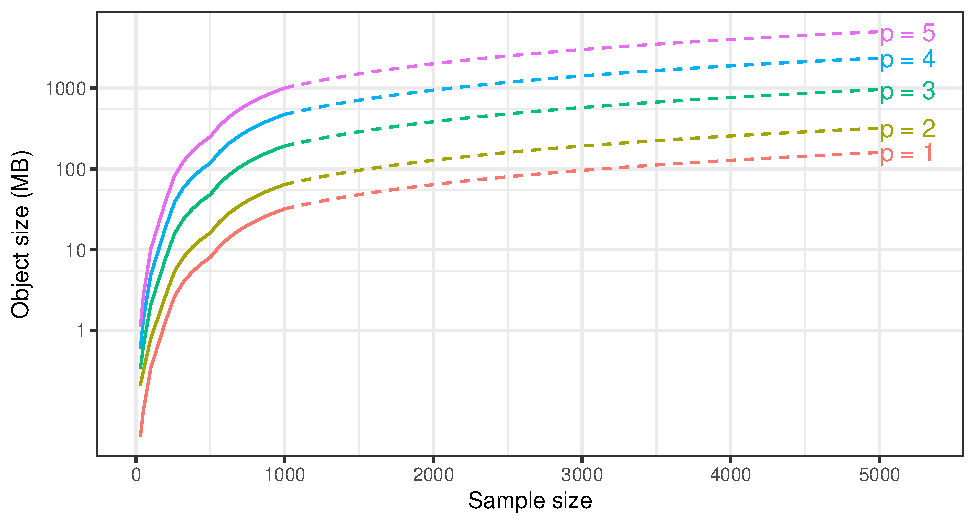
\includegraphics[width=0.85\textwidth]{figure/04-iprior_size}
  \caption[Storage cost of front-loading the kernel matrices.]{Storage cost of front-loading the kernel matrices for varying number of ANOVA components $p=1,\dots,5$ and sample sizes. Solid lines indicate actual values, while dotted lines represent (linear) predictions. Storage requirements increases exponentially, since for $p$ ANOVA components, there are $2^{p+1}$ kernel matrices to store in memory.}
  \label{fig:ipriorstorage}
\end{figure}

\subsection{The exponential family EM algorithm}
\label{sec:expfamEM}

In the original EM paper by \citet{dempster1977maximum}, the EM algorithm was demonstrated to be easily administered to complete data likelihoods belonging to the exponential family for which the maximum likelihood estimates are easily computed.
If this is the case, then the M-step simply involves replacing the unknown sufficient statistics in the ML estimates with their \emph{conditional expectations}.
Certain I-prior models admit this property, namely regression functions belonging to the full or limited ANOVA RKKS.
For such models, we can reduce the EM algorithm to a sequential updating scheme of the latent variables (missing data) and parameters, bypassing the need for a gradient-based optimisation in the M-step.
We describe the implementation of this exponential family EM below.

Assume \ref{ass:A1}--\ref{ass:A3} applies, and that only the error precision $\psi$ and the RKHS scale parameters $\lambda_1,\dots,\lambda_p$ need to be estimated, i.e. all other kernel parameters are fixed---a similar situation was described in the previous subsection.
For the full ANOVA RKKS, the kernel can be written in the form
\begin{align*}
  h_\lambda 
  &= \sum_{i=1}^p \lambda_i h_i + \sum_{i<j} \lambda_i \lambda_j h_i h_j + \cdots + \prod_{i=1}^p \lambda_i h_i \\
  &= \lambda_k 
  \myoverbrace{
  \Bigg(  
  {\color{colblu} h_k + \sum_{i} \lambda_i h_i h_k + \cdots + h_k \prod_{i\neq k} \lambda_i h_i}
  \Bigg)
  }{\text{terms of $\lambda_k$}} 
  + 
  \myoverbrace{\color{colred}
  \phantom{\Bigg(}
  \sum_{i\neq k} \lambda_i h_i + \sum_{i,j \neq k} \lambda_i \lambda_j h_i h_j + \cdots + 0
  }{\text{no $\lambda_k$ here}} \\
  &= \lambda_k {\color{colblu}r_k} + {\color{colred}s_k}
\end{align*}
where $r_k$ and $s_k$ are both functions over $\cX\times\cX$, defined respectively as the terms of the ANOVA kernel involving $\lambda_k$, and the terms not involving $\lambda_k$.
The reason for splitting $h_\lambda$ like this will become apparently momentarily.

Programmatically, this looks complicated to implement in software, but in fact it is not.
Consider again the instruction list $\cQ$ for the ANOVA RKKS (Example 3, \cref{sec:efficientEM1}).
We can split this list into two: $\cR_k$ as those elements of $\cQ$ which involve the index $k$, and $\cS_k$ as those elements of $\cQ$ which do not involve the index $k$.
Let $\zeta_k$, $e_k$ be the sets of $\lambda$ and $h$ after applying the instructions of $\cR_k$, and let $\xi_k$ and $a_k$ be the sets of $\lambda$ and $h$ after application of the instruction list $\cS_k$.
Now, we have 
\[
  r_k = \frac{1}{\lambda_k} \sum_{l=1}^{\abs{\cR_k}} \zeta_{lk} e_{lk} 
  \hspace{0.5cm}\text{and}\hspace{0.5cm}
  s_k = \sum_{l=1}^{\abs{\cS_k}} \xi_{lk} a_{lk},   
\]
as real-valued functions defined over $\cX\times\cX$.
Defining $\bR_k$ and $\bS_k$ as the kernel matrices with $(i,j)$ entries $r_k(x_i,x_j)$ and $s_k(x_i,x_j)$ respectively, for $i,j=1,\dots,n$, we have that
\[
  \bH_\eta^2 = \lambda_k^2\bR_k^2 + \lambda_k \myoverbrace{\big(\bR_k\bS_k + (\bR_k\bS_k)^\top \big)}{\bU_k} + \bS_k^2.
\]

Consider now the full data log-likelihood for $\lambda_k$, $k=1,\dots,p$, conditionally dependent on the rest of the unknown parameters $\lambda_{-k} = \{\lambda_1,\dots,\lambda_p\} \backslash \{ \lambda_k \}$ and $\psi$:
\begin{align}
  L(\lambda_k|\by,\bw,\lambda_{-k},\psi)
  &= \const 
  - \half \tr \Big( (
  \psi\bH_\eta^2 + \psi^{-1}\bI_n
  )\bw\bw^\top \Big)
  + \psi \tilde\by^\top \bH_\eta \bw \label{eq:logliklambdak} \\
  &= \const 
  - \lambda_k^2 \, \half[\psi] \tr(\bR_k^2 \bw\bw^\top)
  + \lambda_k  \left( 
  \psi \tilde\by^\top \bR_k \bw - \half[\psi] \tr(\bU_k \bw\bw^\top)
  \right). \nonumber
\end{align}
Notice that the above likelihood is an exponential family distribution with the natural parameterisation $\beta = (-\lambda_k^2, \lambda_k)$ and sufficient statistics $T_1$ and $T_2$ defined by
\[
  T_1 = \half[\psi] \tr(\bR_k^2 \bw\bw^\top)
  \hspace{0.5cm}\text{and}\hspace{0.5cm}
  T_2 =  \psi\tilde\by^\top \bR_k \bw - \half[\psi]\tr(\bU_k^2 \bw\bw^\top).
\]
This likelihood is maximised at $\hat\lambda_k = T_2/2T_1$, but of course, the variables $w_1,\dots,w_n$ are never observed.
As per the exponential family EM routine, replace occurrences of $\bw$ and $\bw\bw^\top$ with their respective conditional expectations, i.e. $\bw\mapsto\E[\bw|\by] = \wtilde$ and $\bw\bw^\top\mapsto\E[\bw\bw^\top|\by] = \tilde\bV_w + \wtilde\wtilde^\top$ as defined in \cref{eq:posteriorw}.
That the $\lambda_k$'s have closed-form expressions, together with the closed-form expression for $\psi$ in \cref{eq:closedformpsi}, greatly simplifies the EM algorithm.
At the M-step, one simply updates the parameters in turn, and as such, there is no maximisation per se.

The exponential family EM algorithm for ANOVA-type I-prior models is summarised in \cref{alg:EM2}.
It requires $O(n^3)$ computational time at each step, which is spent on computing the matrix inverse in the E-step.
The M-step takes at most $O(n^2)$ time to compute.
\cref{alg:EM2} also requires front-loading of the kernel matrices, which increases storage requirements. 
As a remark, it is not necessary that $h_\lambda$ is the full ANOVA RKKS; any of the examples 1--3 in \cref{sec:efficientEM1} can be estimated using this method, since they are seen as special cases of the ANOVA decomposition.
%This is also true if we decide to drop any of the terms in the ANOVA kernel.

\begin{algorithm}[hbt]
\caption{Exponential family EM for ANOVA-type I-prior models}\label{alg:EM2}
\begin{algorithmic}[1]
  \Procedure{Initialisation}{}
    \State Initialise $\lambda_1^{(0)},\dots,\lambda_p^{(0)}, \psi^{(0)}$
    \State Compute and store matrices as per $\cR_k$ and $\cS_k$.
    \State $t \gets 0$
  \EndProcedure 
  \Statex
  \While{not converged}{}
    \Procedure{E-step}{}
      \State $\wtilde \gets \psi^{(t)} \bH_{\eta^{(t)}} \big(\psi^{(t)} \bH_{\eta^{(t)}}^2 + \psi^{-(t)}\bI_n \big)^{-1} \tilde\by$
      \State $\Wtilde \gets \big(\psi^{(t)} \bH_{\eta^{(t)}}^2 + \psi^{-(t)}\bI_n \big)^{-1} + \wtilde\wtilde^{\top}$
    \EndProcedure
    \Statex
    \Procedure{M-step}{}
      \For{$k=1,\dots,p$}
        \State $T_{1k} \gets \half \tr(\bR_k^2 \Wtilde)$
        \State $T_{2k} \gets \tilde\by^\top \bR_k \wtilde - \half \tr(\bU_k^2 \Wtilde^\top)$
        \State $\lambda_k^{(t+1)} \gets T_{2k} / 2T_{1k}$
      \EndFor
      \State $T_3 \gets \tilde\by^\top\tilde\by + \tr(\bH_{\eta^{(t)}}^2\Wtilde^{(t)}) - 2\tilde\by^\top\bH_{\eta^{(t)}}\wtilde^{(t)}$
      \State $\psi^{(t+1)} \gets \tr \Wtilde^{(t)} / T_3$
    \EndProcedure
    \State $t \gets t+1$
  \EndWhile
\end{algorithmic}
\end{algorithm}

%\bPsi \bH_\eta \bV_y^{-1} (\by - \alpha\bone_n - \bff_0)
%    \hspace{0.5cm}\text{and}\hspace{0.5cm}
%    \tilde\bV_w = \big(\bH_\eta\bPsi\bH_\eta + \bPsi^{-1}\big)^{-1} = \bV_y^{-1},

%For these three examples, the specific form of the matrices $\bR_k$ and $\bS_k$ are given below
%\begin{enumerate}
%  \item \textbf{Single scale parameter}.
%  \[
%    \bR_1 = \bH_1 
%    \hspace{0.5cm}\text{and}\hspace{0.5cm}
%    \bS_1 = \bzero
%  \]
%  \item \textbf{Multiple scale parameters}.
%  \[
%    \bR_k = \bH_k
%    \hspace{0.5cm}\text{and}\hspace{0.5cm}
%    \bS_k = \sum_{j\neq k} \lambda_j \bH_j
%  \]
%  \item \textbf{Multiple scale parameters with level-2 interactions}.
%  \[
%    \bR_k = \bH_k + \sum_{j\neq k} \lambda_j (\bH_j \circ \bH_k)
%    \hspace{0.5cm}\text{and}\hspace{0.5cm}
%    \bS_k = \sum_{j\neq k} \lambda_j \bH_j + \sum_{j<j', j,j' \neq k} \lambda_j\lambda_{j'} (\bH_j \circ \bH_{j'})
%  \]
%\end{enumerate}

\begin{remark}
  Another compelling reason to use \cref{alg:EM2} is conjugacy of the exponential family of distributions.
  Realise that $\lambda_k|(\by,\bw,\lambda_{-k},\psi)$ is in fact normally distributed, with mean and variance given by $T_2/2T_1$ and $1/2T_1$ respectively.
  If we were so compelled to assign a normal prior on each of the $\lambda_k$'s, then the conditionally dependent log-likelihood of $\lambda_k$, $L(\lambda_k|\by,\bw,\lambda_{-k},\psi)$, would have a normal prior log-density involving $\lambda_k$ added on.
  Importantly, viewed as a posterior log-density for $\lambda_k$, the $\lambda_k$ is normally distributed.
  The exponential family EM is thus easily modified to compute maximum a posteriori (MAP) estimates (or penalised ML estimates) of the scale parameters.
  With diffuse priors on $\lambda_k$, MAP estimates are in fact ML estimates.
\end{remark}

\begin{remark}
  The restriction to ANOVA RKKSs is due to the fact that as soon as higher degrees of the $\lambda_k$'s come into play, e.g. using the polynomial kernel, then the ML estimates for the $\lambda_k$'s involve solving a polynomial of degree $2d-1$ for FOC equations.
  Although this is not in itself hard to do, the elegance of the algorithm, especially viewed as having the normal conjugacy property for the $\lambda_k$'s, is lost.
\end{remark}

%\subsection{Accelerating the EM algorithm}
%
%A criticism of the EM algorithm is that it may take many iterations to converge.
%Several novel ideas have been looked at in a bid to `accelerate the EM algorithm', as it were.
%One such approach, which does not require any amendment to the particular EM algorithm at hand, is called the \emph{monotonically over-relaxed EM algorithm} (MOEM) by \citet{yu2012monotonically}.
%
%The idea of MOEM is as follows.
%At every iteration of the MOEM, perform as usual the E-step and M-step to obtain an updated parameter value $\theta^{(t+1)}_\text{EM}$.
%Instead of using this update value of the parameter, modify it instead, and use
%\[
%  \theta^{(t+1)} = (1 + \omega) \theta^{(t+1)}_\text{EM} - \omega \theta^{(t)},
%\]
%where $\omega$ is an \emph{over-relaxation} parameter.
%Under mild conditions, among them that $Q(\theta^{(t+1)}) > Q(\theta^{(t)})$, the MOEM estimate does not decrease the log-likelihood at each step.
%This condition is a slight inconvenience to check under the usual EM algorithm, but is a great companion to exponential family EM algorithm.
%From \cref{eq:logliklambdak}, we see that $Q(\lambda_k) = \E_\bw \big[ L(\lambda_k|\theta\backslash\{\lambda_k \} ) | \by,\theta^{(t)} \big]$ is quadratic in $\lambda_k$, therefore any $\omega \in [0,1]$ will maintain monotonicity of the EM algorithm.
